%Beamer class
\documentclass{beamer}

\usepackage[czech]{babel}
\usepackage[utf8]{inputenc}
\usepackage[T1]{fontenc}
\usepackage{tgheros}
\usepackage{array}
\usepackage{color}
\usepackage{hyperref}
\usepackage{fancyvrb} % pro verbatim
\usepackage{graphicx}

\usetheme{AnnArbor}
\usecolortheme{crane}
\setbeamerfont{description item}{series=\bfseries}


\title[KiCad PCB Editor]{Návrh DPS v KiCad}
\subtitle[KEO]{\texorpdfstring{Konstrukce a realizace elektronických obvodů}{Konstrukce a realizace elektronickych obvodu}}
\author[Brejcha]{\texorpdfstring{Michal Brejcha\newline\url{brejcmic@fel.cvut.cz}}{Michal Brejcha}}
\institute[ČVUT]{ČVUT v Praze, FEL}
\date[Praha, 2026]{Praha, 2026}

%------------------------------------------------------------------------------
%Konstanty a definice
%------------------------------------------------------------------------------
\newtheorem{myDef}{}
\newcommand{\kicadVersion}{10.0}

\begin{document}
%------------------------------------------------------------------------------
%Uvodni slajd
%------------------------------------------------------------------------------
\frame{\titlepage}

\begin{frame}
\frametitle{Obsah} 
\tableofcontents
\end{frame}

\AtBeginSection[]
{
  \begin{frame}
    \frametitle{Téma}
    \tableofcontents[currentsection]
  \end{frame}
}

%------------------------------------------------------------------------------
% Práce v editoru DPS
%------------------------------------------------------------------------------
\section{\texorpdfstring{Práce v editoru DPS}{Prace v editoru DPS}}
%------------------------------------------------------------------------------
\begin{frame}
	\frametitle{Otevření editoru DPS}
	\begin{enumerate}
		\item Ve správci projektu otevřete \textbf{Editor DPS}.
		\item Při prvním spuštění potvrďte doporučené tabulky knihoven.
		\item Uložte desku pomocí \textbf{Ctrl+S} (\texttt{*.kicad\_pcb}).
	\end{enumerate}

	\vfill
	\begin{block}{Výsledek}
		Projekt je připraven pro kreslení DPS.
	\end{block}

\end{frame}

%------------------------------------------------------------------------------
\subsection{\texorpdfstring{Nastavení desky}{Nastaveni desky}}
%------------------------------------------------------------------------------
\begin{frame}{Otevření nastavení desky}
	\begin{enumerate}
		\item V editoru DPS zvolte \textbf{Soubor → Nastavení desky\ldots}
		\item Stejný dialog otevře ikona \textbf{Nastavení desky} v horní nástrojové liště.
		\item Vlevo vyberte stránku nastavení, vpravo upravte hodnoty.
		\item Změny potvrďte tlačítkem \textbf{OK} a desku uložte.
	\end{enumerate}
	\begin{block}{Než začnete kreslit}
	Nejprve zvolte počet vrstev a výrobní pravidla. Rozměry a odstupy přizpůsobte možnostem zvoleného výrobce DPS.
	\end{block}
\end{frame}

%------------------------------------------------------------------------------
\begin{frame}{Nastavení desky: struktura a výroba}
	\small
	\begin{description}
		\item[Vrstvy editoru] Názvy a použití vrstev, zapnutí volitelných vrstev a přidání uživatelských vrstev.
		\item[Fyzická struktura] Počet měděných vrstev, materiály, tloušťky a skladba desky.
		\item[Povrchová úprava desky] Úprava mědi, pokovení hran a další výrobní atributy pro soubor Gerber Job.
		\item[Nepájivá maska / pájecí pasta] Velikost otvorů masky a šablony vůči ploškám, můstky masky a zakrytí prokovů.
		\item[Posuny šrafování zón] Posunutí šrafované výplně v osách X a Y zvlášť pro jednotlivé vrstvy.
	\end{description}
\end{frame}

%------------------------------------------------------------------------------
\begin{frame}{Nastavení desky: text a grafika}
	\begin{description}
		\item[Výchozí hodnoty] Rozměry a vzhled nových textů, tloušťky grafických čar, vlastnosti kót a nových zón.
		\item[Formátování] Vzhled přerušovaných čar a použití výchozích hodnot desky na nově přidaná pouzdra.
		\item[Textové proměnné] Společné texty projektu, např. revize. Zápis \texttt{\$\{REVIZE\}} se nahradí hodnotou proměnné.
	\end{description}
	\begin{block}{Společné se schématem}
	Textové proměnné i třídy spojů jsou sdílené v rámci projektu. Není nutné je vytvářet podruhé.
	\end{block}
\end{frame}

%------------------------------------------------------------------------------
\begin{frame}{Nastavení desky: návrhová pravidla}
	\small
	\begin{description}
		\item[Omezení] Nepodkročitelná minima rozměrů a odstupů pro celou desku.
		\item[Třídy spojů] Odstupy a výchozí rozměry spojů a prokovů pro skupiny sítí.
		\item[Předdefinované velikosti] Nabídka rozměrů pro ruční výběr při routování.
		\item[Kapkovité spoje] Výchozí rozšíření spojů u plošek, prokovů a přechodů šířek.
		\item[Vzory pro ladění délky] Výchozí tvar meandrů pro dorovnávání délek spojů a diferenciálních párů.
		\item[Profily ladění] Geometrie a zpoždění podle vrstvy; podpora návrhu s požadovanou impedancí.
	\end{description}
\end{frame}

%------------------------------------------------------------------------------
\begin{frame}{Nastavení desky: další pravidla a soubory}
	\small
	\begin{description}
		\item[Třídy součástek] Skupiny pouzder pro vlastní pravidla a vícekanálové návrhy; přiřazení lze řídit podmínkami.
		\item[Vlastní pravidla] Speciální podmínky pro vybrané objekty nebo oblasti. Před použitím zkontrolujte syntaxi.
		\item[Závažnost porušení] Určuje, které nálezy DRC jsou chyby, varování nebo ignorované kontroly.
		\item[Vložené soubory] Uložení kopií externích souborů, například 3D modelů či písem, přímo do desky.
		\item[Import nastavení z jiné desky] Převzetí vybraných nastavení z existujícího souboru \texttt{*.kicad\_pcb}.
	\end{description}
\end{frame}

%------------------------------------------------------------------------------
\begin{frame}{Fyzická struktura: skladba desky}
	\begin{columns}[T]
		\begin{column}{0.39\textwidth}
			\small
			\begin{enumerate}
				\item Otevřete \textbf{Fyzická struktura}.
				\item Nastavte počet měděných vrstev; pro běžnou dvouvrstvou desku \textbf{2}.
				\item Zkontrolujte materiály a tloušťky v tabulce.
				\item Ověřte výslednou tloušťku desky.
			\end{enumerate}
			\end{column}
		\begin{column}{0.59\textwidth}
			\centering
			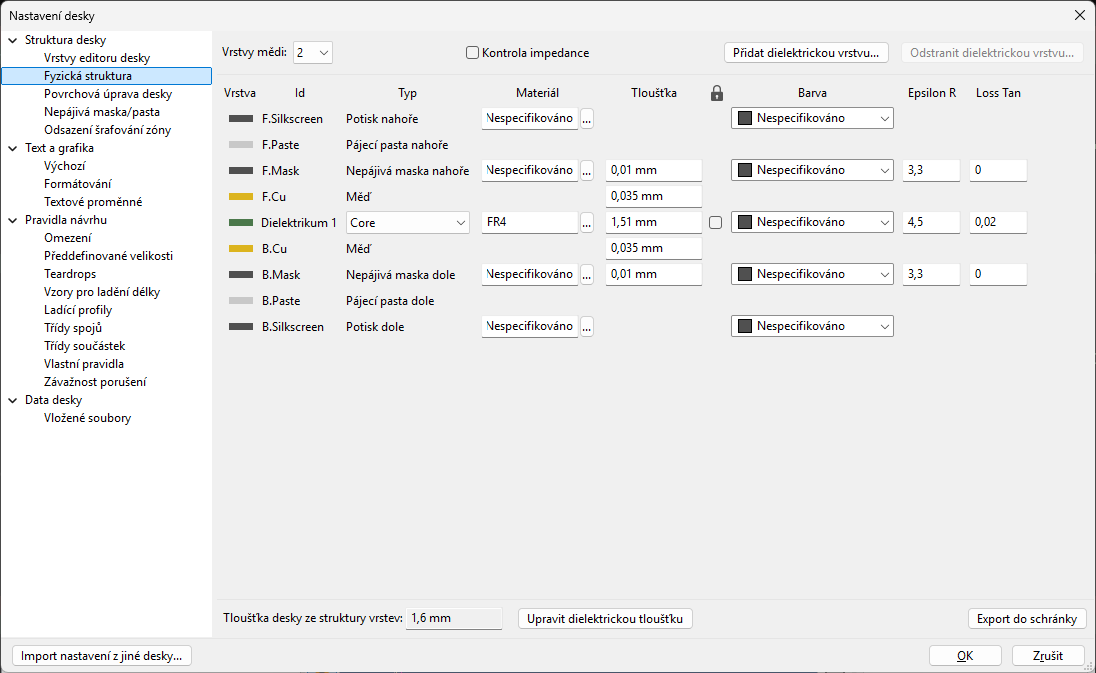
\includegraphics[width=\linewidth,height=0.70\textheight,keepaspectratio]{obr/board_setup_physical_stackup.png}
		\end{column}
	\end{columns}
\end{frame}

%------------------------------------------------------------------------------
\begin{frame}{Fyzická struktura: význam polí}
	\small
	\begin{description}
		\item[Měděné vrstvy] \texttt{F.Cu} je vrchní a \texttt{B.Cu} spodní měď; u vícevrstvé desky přibývají vnitřní vrstvy.
		\item[Dielektrikum] Izolant mezi měděnými vrstvami, typicky FR4. Materiál a tloušťku převezměte ze skladby výrobce.
		\item[Tloušťka mědi] Tloušťka kovu ve vrstvě; ovlivňuje elektrické a tepelné vlastnosti spojů.
		\item[Permitivita a ztráty] Elektrické vlastnosti materiálu důležité zejména pro impedanci a rychlé signály.
		\item[Barva] Barva izolantu, masky a potisku pro 3D zobrazení a export modelu.
	\end{description}
	\begin{block}{Proč zadávat skutečnou skladbu?}
	Tloušťka se promítne do 3D modelu a může se započítávat do délky spojení přes prokovy. Pro řízenou impedanci použijte skladbu výrobce.
	\end{block}
\end{frame}

%------------------------------------------------------------------------------
\begin{frame}{Vrstvy editoru: nastavení}
	\begin{columns}[T]
		\begin{column}{0.39\textwidth}
			\small
			\begin{enumerate}
			\item Otevřete \textbf{Vrstvy editoru}.
			\item Ponechte vrstvy potřebné pro návrh a dokumentaci.
			\item Volitelné nepoužívané vrstvy lze vypnout.
			\item Podle potřeby upravte názvy nebo přidejte uživatelskou vrstvu.
			\end{enumerate}
		\end{column}
		\begin{column}{0.59\textwidth}
			\centering
			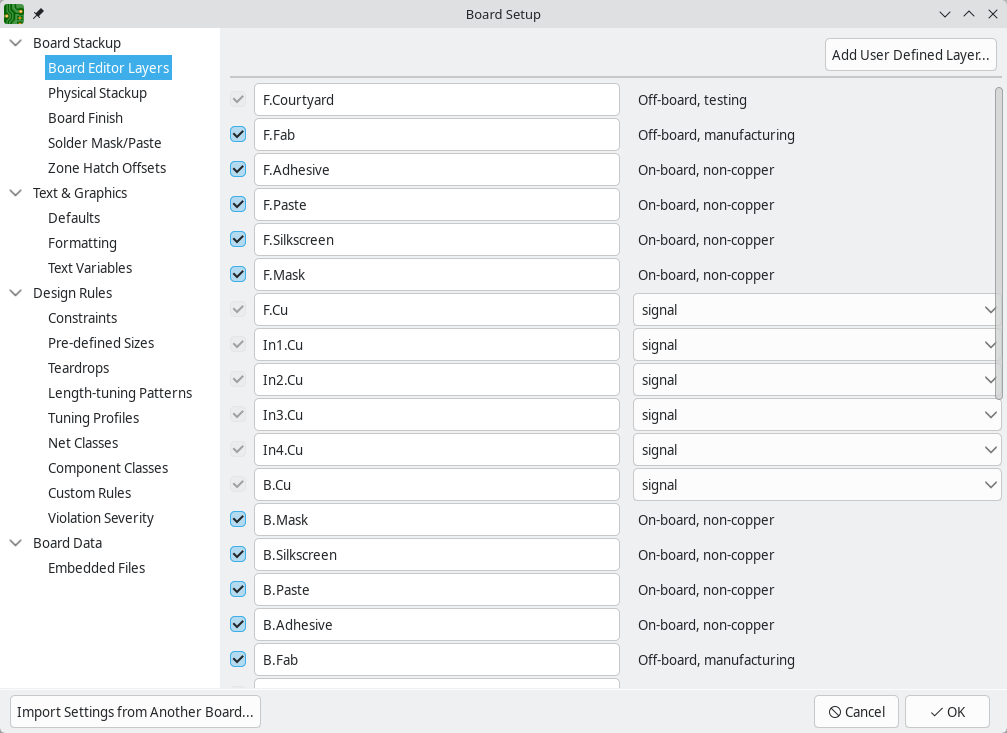
\includegraphics[width=\linewidth,height=0.70\textheight,keepaspectratio]{obr/board_setup_board_editor_layers.png}
		\end{column}
	\end{columns}
\end{frame}

%------------------------------------------------------------------------------
\begin{frame}{Vrstvy editoru: měď, maska a pasta}
	\begin{description}
		\item[F.Cu / B.Cu] Přední a zadní měď: plošky, spoje a měděné zóny.
		\item[F.Mask / B.Mask] Otvory v nepájivé masce. Nakreslený tvar znamená odkrytou měď.
		\item[F.Paste / B.Paste] Otvory šablony pro nanesení pájecí pasty, zejména pro SMD plošky.
		\item[F.Silkscreen / B.Silkscreen] Potisk: reference, označení polarity a další popisky.
		\item[F.Adhesive / B.Adhesive] Podklady pro nanášení lepidla na součástky, pokud to výroba vyžaduje.
	\end{description}
\end{frame}

%------------------------------------------------------------------------------
\begin{frame}{Vrstvy editoru: obrys a dokumentace}
	\small
	\begin{description}
		\item[Edge.Cuts] Uzavřený obrys desky a vnitřních výřezů určených k frézování.
		\item[Margin] Pomocná hranice; sama neurčuje skutečný okraj desky ani automaticky nezakazuje měď.
		\item[F.Courtyard / B.Courtyard] Prostor potřebný pro osazení součástky; pomáhá kontrolovat kolize pouzder.
		\item[F.Fab / B.Fab] Montážní dokumentace: obrysy těles, reference a údaje pro osazení.
		\item[Uživatelské vrstvy] Pomocné výkresy, poznámky a kóty. Nejsou určeny pro routování spojů.
	\end{description}
\end{frame}

%------------------------------------------------------------------------------
\begin{frame}{Vrstvy editoru: co nastavení mění}
	\begin{itemize}
		\item Počet měděných vrstev nastavujte ve \textbf{Fyzické struktuře}.
		\item Povinné vrstvy, např. měď, \texttt{Edge.Cuts} a vrstvy \texttt{Courtyard}, nelze vypnout.
		\item Typ měděné vrstvy (signálová, napájecí apod.) slouží jako informace pro návrháře; neomezuje kreslení spojů a zón.
		\item \textbf{Skrytí vrstvy} v panelu Vzhled mění pouze zobrazení. Obsah vrstvy zůstává součástí desky.
	\end{itemize}
	\begin{block}{Při kreslení}
	Aktivní vrstva určuje, kam se vloží nový objekt. Před kreslením vždy zkontrolujte její název.
	\end{block}
\end{frame}

%------------------------------------------------------------------------------
\begin{frame}{Omezení: výrobní minima}
	\begin{columns}[T]
		\begin{column}{0.39\textwidth}
			\small
			\begin{enumerate}
				\item Otevřete \textbf{Návrhová pravidla → Omezení}.
				\item Zjistěte minimální rozměry a odstupy u výrobce.
				\item Zadejte je jako globální minima desky.
			\end{enumerate}
			\medskip
			Třídy spojů ani vlastní pravidla tato minima nesmějí snížit.
			\end{column}
		\begin{column}{0.59\textwidth}
			\centering
			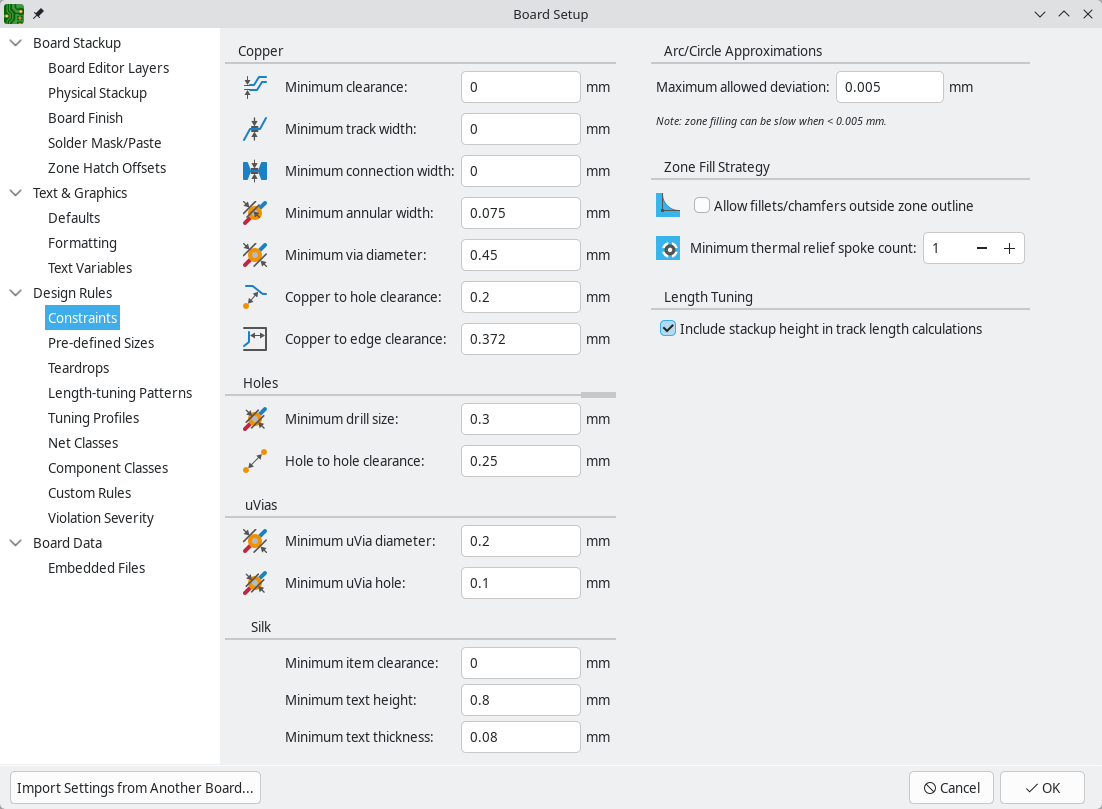
\includegraphics[width=\linewidth,height=0.70\textheight,keepaspectratio]{obr/board_setup_constraints.png}
		\end{column}
	\end{columns}
\end{frame}

%------------------------------------------------------------------------------
\begin{frame}{Omezení: měď a otvory}
	\small
	\begin{description}
		\item[Minimální odstup mědi] Nejmenší mezera mezi vodivými cestami různých sítí.
		\item[Minimální šířka spoje] Nejtenčí dovolený měděný spoj na desce.
		\item[Měď vůči okraji / otvoru] Odstup mědi od hrany desky a od otvorů podle příslušné kontroly.
		\item[Minimální průměr prokovu] Vnější průměr měděné plošky prokovu.
		\item[Minimální mezikruží] Šířka mědi kolem vrtání; pro kruhový prokov přibližně $(D-d)/2$.
		\item[Minimální vrtání a rozteč otvorů] Nejmenší mechanicky vrtaný otvor a mezera mezi hranami otvorů.
	\end{description}
\end{frame}

%------------------------------------------------------------------------------
\begin{frame}{Omezení: další kontroly a volby}
	\small
	\begin{description}
		\item[Mikroprokovy a speciální prokovy] Použití a rozměry nastavujte pouze pro technologii, kterou výrobce podporuje.
		\item[Potisk] Minimální výška a tloušťka textu, mezery mezi prvky a odstup potisku od otvorů masky.
		\item[Tepelné můstky] Minimální počet můstků připojujících plošku k měděné zóně.
		\item[Aproximace oblouků] Největší odchylka při nahrazení oblouku úsečkami; menší hodnota zvyšuje náročnost výpočtu.
		\item[Zaoblení mimo obrys zóny] Povoluje přesah mědi při zaoblení vnitřních rohů zóny.
		\item[Výška skladby v délce spojů] Zahrnutí svislé délky prokovů do výpočtu délky spojení.
	\end{description}
\end{frame}

%------------------------------------------------------------------------------
\begin{frame}{Omezení: výroba v JLCPCB}
	\small
	Společné konzervativní nastavení pro levnou \textbf{2vrstvou i 4vrstvou FR4 DPS}, rozměry nejvýše \textbf{100\,$\times$\,100 mm}.
	\begin{center}
		\begin{tabular}{lr}
			\textbf{Omezení v KiCadu} & \textbf{Nastavit} \\
			\hline
			Minimální šířka spoje & 0,15 mm \\
			Minimální odstup mědi & 0,15 mm \\
			Minimální průměr prokovu & 0,60 mm \\
			Minimální vrtání & 0,30 mm \\
			Minimální mezikruží prokovu & 0,15 mm \\
			Měď od frézovaného okraje & 0,30 mm \\
			Měď od cizího otvoru & 0,35 mm \\
			Odstup mezi hranami vrtání & 0,50 mm \\
		\end{tabular}
	\end{center}
	\begin{block}{Pravidla pro cvičení}
	Jde o zvolené hodnoty s rezervou, nikoli o technologická minima JLCPCB. Pro běžné spoje používejte šířku 0,25 mm nebo větší.
	\end{block}
	\vfill
	{\tiny Zdroj: \href{https://jlcpcb.com/capabilities/pcb-capabilities}{JLCPCB -- PCB Capabilities}, ověřeno 17.\,10.\,2026.}
\end{frame}

%------------------------------------------------------------------------------
\begin{frame}{JLCPCB: otvory a potisk bez zvláštních požadavků}
	\small
	\begin{itemize}
		\item Použijte běžné \textbf{průchozí prokovy 0,60/0,30 mm} (vnější průměr / vrtání), bez výplně a překovení.
		\item Otvory pro vývody součástek: mezikruží alespoň \textbf{0,25 mm}; např. vrtání 0,80 mm a ploška 1,30 mm. Nezaměňujte s mezikružím prokovu.
		\item Nepokovené otvory nejméně \textbf{0,50 mm}; výřezy navrhujte široké \textbf{nad 1 mm} a omezte jejich počet.
		\item Potisk: výška textu alespoň \textbf{1 mm}, tloušťka tahu \textbf{0,15 mm}, odstup od plošek alespoň \textbf{0,15 mm}.
	\end{itemize}
	\begin{block}{Malé vrtání nemusí být zdarma}
	Vrtání 0,15 mm je příplatkové. U vícevrstvých desek je 0,20 mm bez příplatku při vnějším průměru prokovu alespoň 0,45 mm. Pro cvičení ponechte vrtání 0,30 mm.
	\end{block}
	\vfill
	{\tiny Zdroje: \href{https://jlcpcb.com/capabilities/pcb-capabilities}{PCB Capabilities}, \href{https://cart.jlcpcb.com/quote}{kalkulátor JLCPCB}; ověřeno 17.\,10.\,2026.}
\end{frame}

%------------------------------------------------------------------------------
\begin{frame}{JLCPCB: zachování základní ceny objednávky}
	\small
	\begin{itemize}
		\item \textbf{Jeden návrh, samostatná deska, 5 kusů}; oba rozměry nejvýše \textbf{100 mm}. Bez panelizace, V-drážek a odlamovacích můstků.
		\item \textbf{FR4, 2 nebo 4 vrstvy, tloušťka 1,6 mm}, zelená maska, bílý potisk; standardní skladba výrobce.
		\item Vnější měď \textbf{1 oz}, u 4 vrstev vnitřní měď \textbf{0,5 oz}; povrch \textbf{HASL}, nejlevnější varianta v kalkulátoru.
		\item Bez ENIG, pokovení hran, půlotvorů, slepých prokovů, výplně pryskyřicí a expresní výroby. Ponechte výrobní označení JLCPCB.
		\item Nejvýše \textbf{150\,000 vrtání/m$^2$}: \textbf{1\,500 otvorů na 100\,$\times$\,100 mm}, u menší desky úměrně méně.
	\end{itemize}
	\begin{block}{Kontrola ceny}
	Po nahrání Gerberů ověřte cenu pro zvolený počet vrstev. Akce se mění; doprava a daně se účtují zvlášť.
	\end{block}
	\vfill
	{\tiny Zdroje: \href{https://jlcpcb.com/help/article/in-what-cases-will-there-be-charged-extra}{JLCPCB -- příplatky}, \href{https://cart.jlcpcb.com/quote}{kalkulátor}; ověřeno 17.\,10.\,2026.}
\end{frame}

%------------------------------------------------------------------------------
\begin{frame}{Třídy spojů: skupiny sítí}
	\begin{columns}[T]
		\begin{column}{0.39\textwidth}
		\small
		\begin{enumerate}
			\item Otevřete \textbf{Třídy spojů}.
			\item Zkontrolujte třídy převzaté ze schématu.
			\item Tlačítkem \textbf{+} přidejte potřebnou třídu.
			\item Vyplňte parametry a přiřaďte sítě.
		\end{enumerate}
		\end{column}
		\begin{column}{0.59\textwidth}
			\centering
			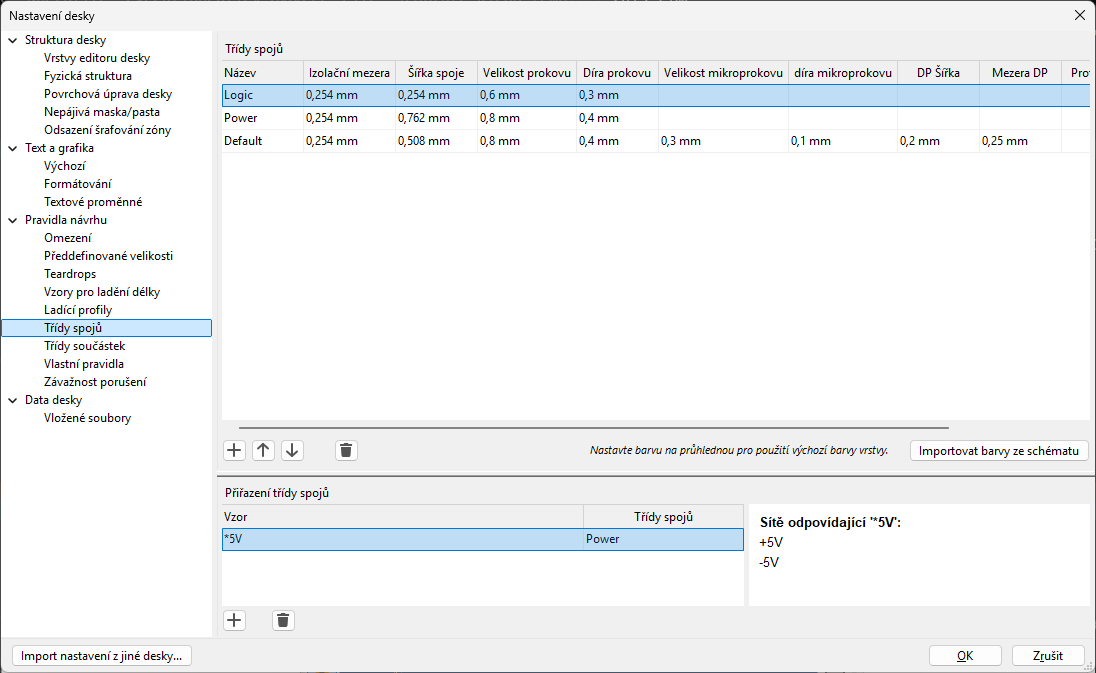
\includegraphics[width=\linewidth,height=0.70\textheight,keepaspectratio]{obr/board_setup_netclasses.png}
		\end{column}
	\end{columns}
\end{frame}

%------------------------------------------------------------------------------
\begin{frame}{Třídy spojů: význam sloupců}
	\small
	\begin{description}
		\item[Odstup] Požadovaná mezera mědi vůči jiným sítím; při rozdílných požadavcích se uplatní přísnější odstup.
		\item[Šířka spoje] Výchozí šířka při routování s volbou použití hodnot třídy.
		\item[Průměr / vrtání prokovu] Vnější průměr měděné plošky a průměr otvoru; zvlášť lze definovat mikroprokovy.
		\item[Diferenciální pár] Šířka jednotlivých vodičů, mezera mezi nimi a mezera prokovů páru.
		\item[Barva PCB] Volitelné zvýraznění sítí dané třídy podle nastavení panelu Vzhled.
		\item[Profil ladění] Volitelná geometrie a zpoždění podle vrstvy pro náročnější signály.
	\end{description}
\end{frame}

%------------------------------------------------------------------------------
\begin{frame}{Třídy spojů: přiřazení sítí}
	\begin{enumerate}
		\item Pro běžné signály ponechte třídu \textbf{Default}.
		\item Vytvořte například třídu \textbf{POWER} pokud ještě neexistuje.
		\item V dolní tabulce přidejte pravidlo: vzor \texttt{+5V}, třída \texttt{POWER}.
		\item Pro více podobných názvů lze použít zástupné znaky, např. \texttt{PWR\_*}.
		\item Zkontrolujte, že vzor odpovídá skutečným názvům sítí. Přiřazení může být určeno také ve schématu.
	\end{enumerate}
	\begin{block}{Návaznost na schéma}
	Třídu lze přiřadit popiskem nebo direktivou ve schématu. Při práci používejte jeden společný projekt.
	\end{block}
\end{frame}

%------------------------------------------------------------------------------
\begin{frame}{Třídy spojů: příklad a význam hodnot}
	\begin{center}
		\begin{tabular}{lrrr}
			\textbf{Třída} & \textbf{Odstup} & \textbf{Šířka} & \textbf{Prokov / vrtání} \\
			\hline
			Default & 0,20 mm & 0,25 mm & 0,60 / 0,30 mm \\
			POWER & 0,25 mm & 0,50 mm & 0,80 / 0,40 mm \\
		\end{tabular}
	\end{center}
	\small
	\begin{itemize}
		\item Hodnoty jsou ilustrativní; šířku napájecích spojů určete podle proudu a dovoleného oteplení.
		\item Šířka a velikost prokovu ve třídě jsou \textbf{výchozí hodnoty}, nikoli pevně vynucené rozměry.
		\item Jiná ručně zvolená šířka sama o sobě neznamená chybu DRC. Pevné požadavky lze vynutit vlastními pravidly.
		\item Globální minima z \textbf{Omezení} platí vždy.
	\end{itemize}
\end{frame}

%------------------------------------------------------------------------------
\begin{frame}{Předdefinované velikosti: doplnění nabídky při routování}
	\begin{columns}[T]
		\begin{column}{0.39\textwidth}
			\small
			\begin{enumerate}
				\item Otevřete \textbf{Předdefinované velikosti}.
				\item Přidejte používané šířky spojů.
				\item Přidejte dvojice průměr / vrtání prokovu.
				\item Pro diferenciální páry zadejte šířku a příslušné mezery.
			\end{enumerate}
		\end{column}
		\begin{column}{0.59\textwidth}
			\centering
			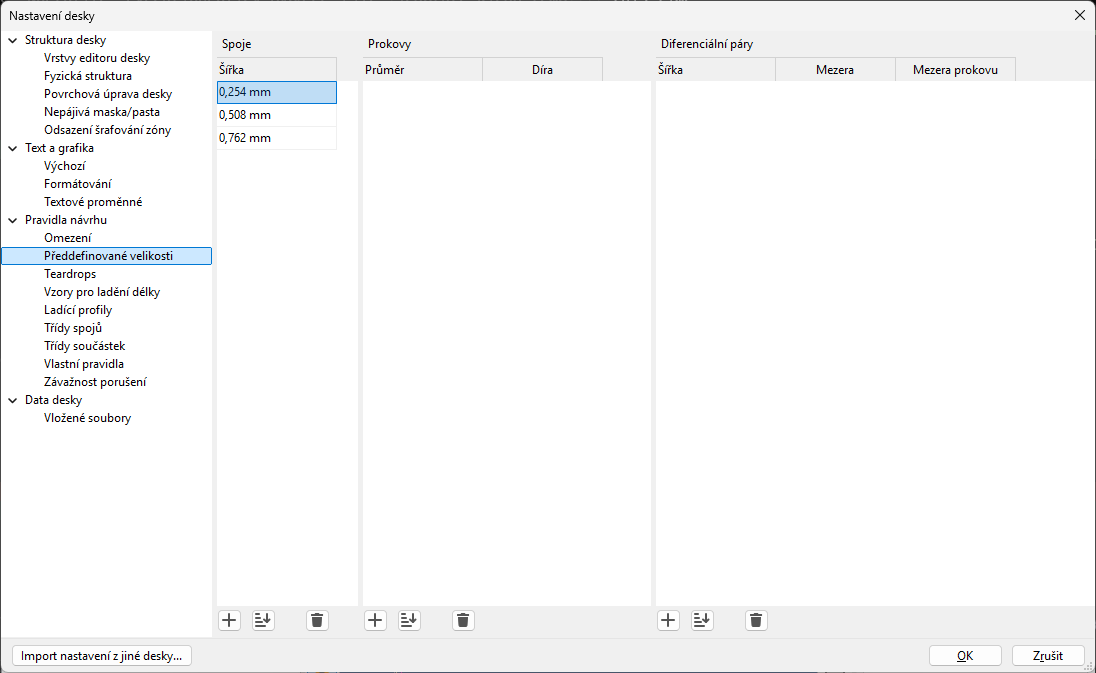
\includegraphics[width=\linewidth,height=0.70\textheight,keepaspectratio]{obr/board_setup_predefined_sizes.png}
		\end{column}
	\end{columns}
\end{frame}

%------------------------------------------------------------------------------
\begin{frame}{Kontrola nastavení před návrhem}
	\begin{enumerate}
		\item \textbf{Fyzická struktura}: odpovídají počet vrstev a tloušťka zadání?
		\item \textbf{Vrstvy editoru}: jsou připraveny měď, maska, potisk a obrys?
		\item \textbf{Omezení}: odpovídají minima technologii výrobce?
		\item \textbf{Třídy spojů}: mají sítě správné přiřazení a výchozí rozměry?
		\item \textbf{Předdefinované velikosti}: obsahuje nabídka potřebné rozměry?
		\item Potvrďte \textbf{OK} a uložte projekt pomocí \textbf{Ctrl+S}.
	\end{enumerate}
\end{frame}

%------------------------------------------------------------------------------
\subsection{\texorpdfstring{Aktualizace DPS ze schématu}{Aktualizace DPS ze schematu}}
%------------------------------------------------------------------------------
\begin{frame}{Aktualizace DPS ze schématu}
	\begin{enumerate}
		\item Ve schématu zkontrolujte reference, přiřazení pouzder a výsledek ERC. Schéma uložte pomocí \textbf{Ctrl+S}.
		\item Otevřete Editor DPS stejného projektu.
		\item Zvolte \textbf{Nástroje → Aktualizovat DPS ze schématu\ldots}, stiskněte \textbf{F8} nebo použijte ikonu v horní liště:
	\end{enumerate}
	\begin{center}
		
\includegraphics[height=0.65cm]{obr/update_pcb_from_schematic_icon.png}
		\quad\textbf{Aktualizovat DPS ze schématu}
	\end{center}
	\begin{block}{Přímý přenos v projektu}
	Přenáší pouzdra, pole a elektrické sítě. Samostatný soubor netlistu při tomto postupu nepotřebujete.
	\end{block}
\end{frame}

%------------------------------------------------------------------------------
\begin{frame}{Aktualizační okno}
	\centering
	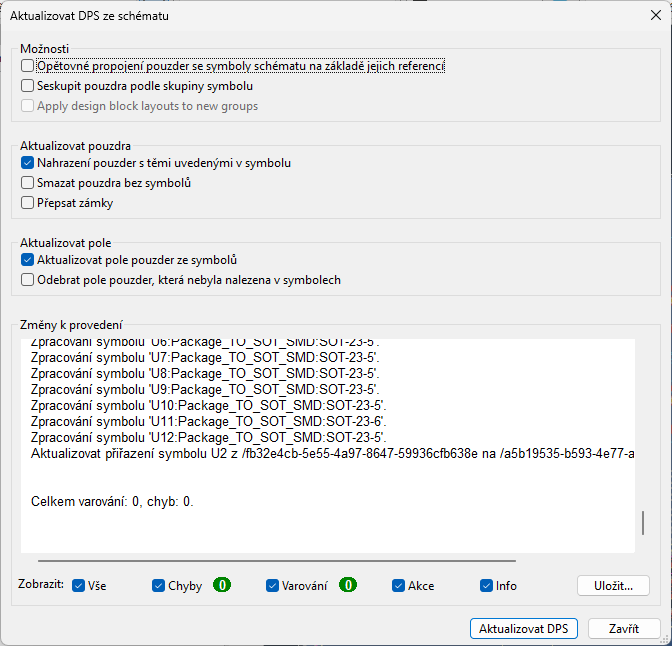
\includegraphics[width=\linewidth,height=0.82\textheight,keepaspectratio]{obr/update_pcb_from_schematic_cs.png}
\end{frame}

%------------------------------------------------------------------------------
\begin{frame}{Aktualizace: propojení a skupiny}
	\begin{description}
		\item[Opětovné propojení podle referencí] Páruje symbol a pouzdro podle označení, např. R1. Běžně ponechte \textbf{vypnuté}: KiCad používá jejich jedinečné identifikátory.
		\item[Seskupit pouzdra podle skupiny symbolu] Přenese seskupení symbolů do skupin pouzder na DPS.
		\item[Apply design block layouts to new groups] Volba pro přenos rozmístění z návrhových bloků. Pro běžný přenos schématu ji nepotřebujete.
	\end{description}
	\begin{block}{Kdy obnovit propojení podle referencí?}
	Například po smazání a opětovném vložení symbolu se stejnou referencí. Nejprve ověřte správné párování; při další běžné aktualizaci volbu opět vypněte.
	\end{block}
\end{frame}

%------------------------------------------------------------------------------
\begin{frame}{Aktualizace: nahrazení a mazání pouzder}
	\begin{description}
		\item[Nahrazení pouzder těmi uvedenými v symbolu] Promítne změnu přiřazeného pouzdra ze schématu také do existující DPS.
		\item[Smazat pouzdra bez symbolů] Odstraní pouzdra, která již nemají odpovídající symbol. Pouzdra s atributem \textbf{Není ve schématu} zůstanou.
		\item[Přepsat zámky] Dovolí nahradit nebo odstranit i uzamčená pouzdra. Zapínejte pouze záměrně.
	\end{description}
	\begin{block}{Před potvrzením}
	Zkontrolujte plánovaná nahrazení a odstranění. Změna pouzdra může vyžadovat úpravu jeho okolních spojů.
	\end{block}
\end{frame}

%------------------------------------------------------------------------------
\begin{frame}{Aktualizace: pole a seznam změn}
	\small
	\begin{description}
		\item[Aktualizovat pole pouzder ze symbolů] Přenese nové a změněné hodnoty polí.
		\item[Odebrat pole nenalezená v symbolech] Smaže dodatečná pole pouzdra, která ve schématu nejsou. Vypněte, pokud je chcete na DPS zachovat.
		\item[Změny k provedení] Výpis plánovaných akcí a případných problémů. Před aktualizací opravte chyby a posuďte varování.
		\item[Zobrazit] Filtry \textbf{Chyby, Varování, Akce, Info} mění zobrazení výpisu, nikoli rozsah aktualizace.
		\item[Uložit\ldots] Uloží zprávu o změnách do souboru; neukládá tím desku.
	\end{description}
	\begin{block}{Rozhodující tlačítka}
	\textbf{Aktualizovat DPS} provede změny. \textbf{Zavřít} ukončí dialog; již provedenou aktualizaci nevrací zpět.
	\end{block}
\end{frame}

%------------------------------------------------------------------------------
\begin{frame}{Aktualizace: dokončení a kontrola}
	\begin{enumerate}
		\item Projděte výpis a stiskněte \textbf{Aktualizovat DPS}.
		\item Zavřete dialog. Nová pouzdra umístěte kliknutím do pracovní plochy; následně je rozmístěte jednotlivě.
		\item Zkontrolujte reference, pouzdra a pomocné čáry propojení (ratsnest).
		\item Po změně schématu upravte také dotčené spoje a zóny.
		\item Desku uložte pomocí \textbf{Ctrl+S}; po dokončení úprav spusťte kontrolu \textbf{DRC}.
	\end{enumerate}
	\begin{block}{Aktualizace nenavrhuje spoje}
	Přenos určí, které plošky mají být propojené. Rozmístění nových pouzder a vedení spojů provede návrhář.
	\end{block}
\end{frame}

%------------------------------------------------------------------------------
\begin{frame}{Alternativa: přenos pomocí netlistu}
	\begin{enumerate}
		\item V editoru schématu zvolte \textbf{Soubor → Exportovat → Netlist\ldots}
		\item Vyberte formát \textbf{KiCad} a uložte soubor \texttt{*.net}.
		\item V Editoru DPS zvolte \textbf{Soubor → Importovat → Netlist\ldots} a načtěte jej.
		\item Zkontrolujte navržené změny, proveďte aktualizaci a rozmístěte nová pouzdra.
	\end{enumerate}
	\begin{block}{Kdy použít netlist?}
	Například při odděleném předávání schématu a DPS. Po změně schématu je nutné netlist znovu exportovat a načíst. V jednom projektu používejte přímou aktualizaci \textbf{F8}.
	\end{block}
	\vfill
	{\tiny Postup: \href{https://docs.kicad.org/10.0/en/pcbnew/pcbnew.html}{KiCad 10 -- PCB Editor}, \href{https://docs.kicad.org/10.0/en/eeschema/eeschema.html}{Schematic Editor}.}
\end{frame}

%------------------------------------------------------------------------------
% Generování výrobních podkladů - Gerber
%------------------------------------------------------------------------------
\section{\texorpdfstring{Generování výrobních podkladů}{Generování výrobních podkladů}}
%------------------------------------------------------------------------------

\end{document}
